%!TEX program = xelatex

\documentclass[11pt,titlepage]{report}
%!TEX root = main.tex

\usepackage[T1]{fontenc}
\usepackage{lmodern}
\usepackage[svgnames]{xcolor}
\usepackage{fontspec} % XeLaTeX required!
\usepackage{graphicx}
\usepackage{circuitikz}
\usepackage{tikz}
\usepackage{pifont}
\usepackage[some]{background}
\usepackage{xltxtra} 
\usepackage{setspace}
\usepackage[absolute]{textpos}
\usepackage[latin1]{inputenc}
\usepackage[english]{babel}
\usepackage{graphicx}
\usepackage{wrapfig}
\usepackage{fullpage}
\usepackage[margin=1in]{geometry}
\usepackage{float}
\usepackage{url}
\usepackage{multicol}
\usepackage{hyperref}
\usepackage{titlepic}
\usepackage{standalone}
\usepackage{siunitx}
\usepackage{booktabs}
\usepackage{amsmath}
\usepackage{unicode-math}
\usepackage{verbatim}
\usepackage{enumitem}
\usepackage{listings}
\usepackage{multirow}
\usepackage{pgfplots}
\pgfplotsset{compat=1.8}
\usepackage{caption} 
\usepackage[parfill]{parskip}
\usepackage{import}
\usepackage[backend=bibtexu,texencoding=utf8,bibencoding=utf8,style=ieee,sortlocale=en_GB,language=auto]{biblatex}
\usepackage[strict,autostyle]{csquotes}
\usepackage[final]{pdfpages}
\usepackage{subcaption}
\usepackage{ifplatform}
%\captionsetup[table]{skip=10pt}


% Fix for includepdf bug in Mac OS X
\newcommand{\insertpdfpath}[1]{
	\ifwindows
	\newcommand{\insertpdf}[2]{\includepdf[pages=##1]{##2}}
	\else
	\newcommand{\insertpdf}[2]{\includepdf[pages=##1]{#1/##2}}
	\fi
}

%set fonts
\setmainfont[Ligatures=TeX]{Myriad Pro}
\setmathfont{Asana Math}
\setmonofont{Lucida Console}

\usepackage{titlesec, color}
\renewcommand{\familydefault}{\sfdefault} %set font family
\renewcommand{\arraystretch}{1.2} %set table vertical spacing
\setlength\parindent{0pt} %no paragraph indent
\hypersetup{ %setup hyperlinks
    colorlinks,
    citecolor=black,
    filecolor=black,
    linkcolor=black,
    urlcolor=black
}

%redesign chapter headings
\definecolor{gray75}{gray}{0.75}
\newcommand{\chapternumber}{\thechapter}
\newcommand{\hsp}{\hspace{20pt}}
\titleformat{\chapter}[hang]{\Huge\bfseries}{\chapternumber\hsp\textcolor{gray75}{|}\hsp}{0pt}{\Huge\bfseries}

%Redefine appendix headers
\renewcommand{\appendixname}{Appendix}
\renewcommand{\appendixtocname}{Appendices}
\renewcommand{\appendixpagename}{Appendices}

%For code listings
\definecolor{black}{rgb}{0,0,0}
\definecolor{browntags}{rgb}{0.65,0.1,0.1}
\definecolor{bluestrings}{rgb}{0,0,1}
\definecolor{graycomments}{rgb}{0.4,0.4,0.4}
\definecolor{redkeywords}{rgb}{1,0,0}
\definecolor{bluekeywords}{rgb}{0.13,0.13,0.8}
\definecolor{greencomments}{rgb}{0,0.5,0}
\definecolor{redstrings}{rgb}{0.9,0,0}
\definecolor{purpleidentifiers}{rgb}{0.01,0,0.01}


\lstdefinestyle{csharp}{
language=[Sharp]C,
showspaces=false,
showtabs=false,
breaklines=true,
showstringspaces=false,
breakatwhitespace=true,
escapeinside={(*@}{@*)},
columns=fullflexible,
commentstyle=\color{greencomments},
keywordstyle=\color{bluekeywords}\bfseries,
stringstyle=\color{redstrings},
identifierstyle=\color{purpleidentifiers},
basicstyle=\ttfamily\small}

\lstdefinestyle{c}{
language=C,
showspaces=false,
showtabs=false,
breaklines=true,
showstringspaces=false,
breakatwhitespace=true,
escapeinside={(*@}{@*)},
columns=fullflexible,
commentstyle=\color{greencomments},
keywordstyle=\color{bluekeywords}\bfseries,
stringstyle=\color{redstrings},
identifierstyle=\color{purpleidentifiers},
}

\lstdefinestyle{matlab}{
language=Matlab,
showspaces=false,
showtabs=false,
breaklines=true,
showstringspaces=false,
breakatwhitespace=true,
escapeinside={(*@}{@*)},
columns=fullflexible,
commentstyle=\color{greencomments},
keywordstyle=\color{bluekeywords}\bfseries,
stringstyle=\color{redstrings},
identifierstyle=\color{purpleidentifiers}
}

\lstdefinestyle{vhdl}{
language=VHDL,
showspaces=false,
showtabs=false,
breaklines=true,
showstringspaces=false,
breakatwhitespace=true,
escapeinside={(*@}{@*)},
columns=fullflexible,
commentstyle=\color{greencomments},
keywordstyle=\color{bluekeywords}\bfseries,
stringstyle=\color{redstrings},
identifierstyle=\color{purpleidentifiers}
}

\lstdefinestyle{xaml}{
language=XML,
showspaces=false,
showtabs=false,
breaklines=true,
showstringspaces=false,
breakatwhitespace=true,
escapeinside={(*@}{@*)},
columns=fullflexible,
commentstyle=\color{greencomments},
keywordstyle=\color{redkeywords},
stringstyle=\color{bluestrings},
tagstyle=\color{browntags},
morestring=[b]",
  morecomment=[s]{<?}{?>},
  morekeywords={xmlns,version,typex:AsyncRecords,x:Arguments,x:Boolean,x:Byte,x:Char,x:Class,x:ClassAttributes,x:ClassModifier,x:Code,x:ConnectionId,x:Decimal,x:Double,x:FactoryMethod,x:FieldModifier,x:Int16,x:Int32,x:Int64,x:Key,x:Members,x:Name,x:Object,x:Property,x:Shared,x:Single,x:String,x:Subclass,x:SynchronousMode,x:TimeSpan,x:TypeArguments,x:Uid,x:Uri,x:XData,Grid.Column,Grid.ColumnSpan,Click,ClipToBounds,Content,DropDownOpened,FontSize,Foreground,Header,Height,HorizontalAlignment,HorizontalContentAlignment,IsCancel,IsDefault,IsEnabled,IsSelected,Margin,MinHeight,MinWidth,Padding,SnapsToDevicePixels,Target,TextWrapping,Title,VerticalAlignment,VerticalContentAlignment,Width,WindowStartupLocation,Binding,Mode,OneWay,xmlns:x}
}

\lstdefinestyle{matlab}{
language=Matlab,
showspaces=false,
showtabs=false,
breaklines=true,
showstringspaces=false,
breakatwhitespace=true,
escapeinside={(*@}{@*)},
columns=fullflexible,
commentstyle=\color{greencomments},
keywordstyle=\color{bluekeywords}\bfseries,
stringstyle=\color{purpleidentifiers},
identifierstyle=\color{purpleidentifiers}
}

%defaults
\lstset{
basicstyle=\ttfamily\small,
extendedchars=false,
numbers=left,
numberstyle=\ttfamily\tiny,
stepnumber=1,
tabsize=4,
numbersep=5pt
}
\addbibresource{../../library/bibliography.bib}

\begin{document}

\chapter{Assignment 4}
\section{Task 1}

\begin{enumerate}
\item
	\begin{itemize}
		\item
		Simulation results indicate the Nissan Leaf is able to accelerate from \num{0} to \SI{60}{mph} (\SI{96.6}{km/h}) in about \num{7.8} seconds. This is lower than the manufacturer's claim, which is peculiar, since manufacturer's claims tend to be quite optimistic. This could be due to the fact the actual transmission efficiency is unknown, but assumed to be \SI{90}{\percent} in our simulation. This, along with other assumptions while simplifying the model, could add up to result in the difference in acceleration times we observe.

		\item
		When looking at the various simulation output graphs, we could see that the engine's torque immediately saturates at its maximum value of \SI{280}{Nm}. Would this value have been higher, the car would have accelerated faster. The electric motor in the car is therefore the limiting component.

		\item
		In de Simulink model, an amplifier (`Driver') with an `infinite' gain is used to determine if the car should accelerate or brake. Since this amplifier has an actual gain of `only' \num{1000}, the car stops accelerating a little under the requested velocity, causing a small steady-state error.
	\end{itemize}

\item
	\begin{itemize}
		\item
		When looking at the various resistance graphs (Figure \ref{fig:ass4-t1-resistance}) we observe nothing out of the ordinary. Aerodynamic drag in- and decreases nicely with vehicle speed and friction is a constant value when vehicle velocity is greater than zero and zero otherwise. The gravitational force is at a constant zero, since there is no inclination in our simulation.

		\begin{figure}[H]
			\begin{center}
				\begin{subfigure}[h]{0.49\textwidth}
					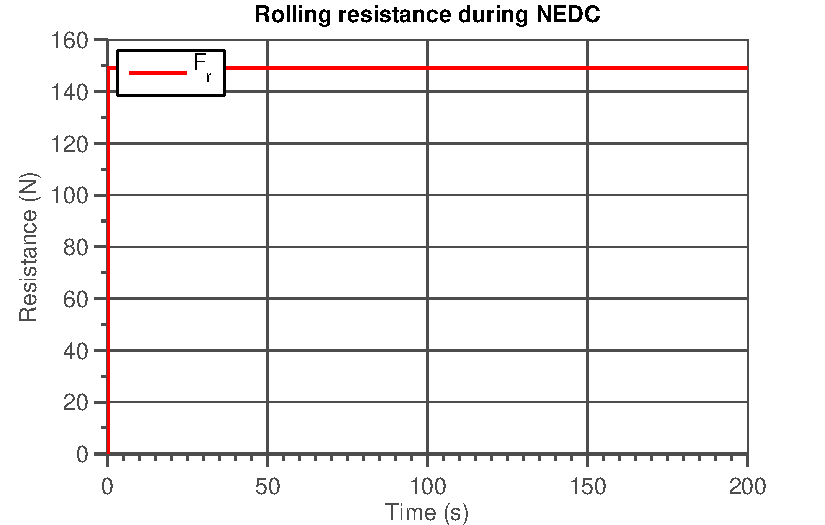
\includegraphics[width=\textwidth]{resource/leaf/resistance-friction-rc.pdf}
					\caption{Nissan Leaf Frictional Resistance}
					\label{fig:ass4-t1-resistance-friction}
				\end{subfigure}
				\enspace
				\begin{subfigure}[h]{0.49\textwidth}
					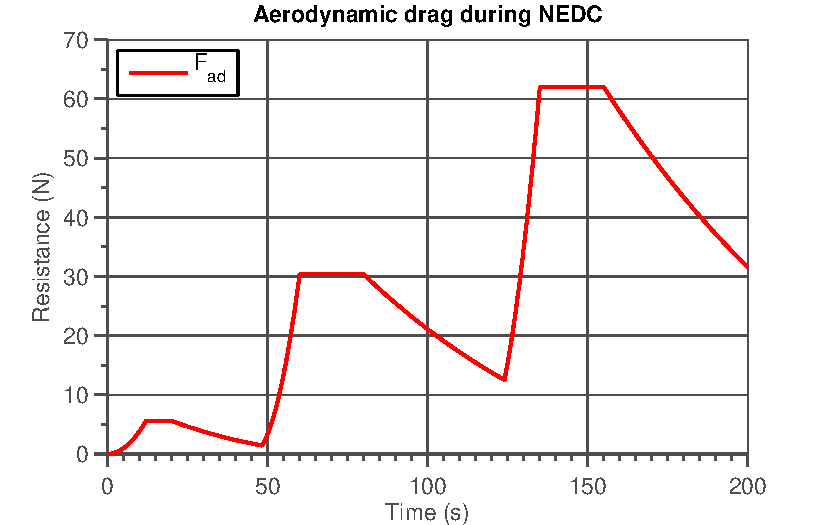
\includegraphics[width=\textwidth]{resource/leaf/resistance-aero-rc.pdf}
					\caption{Nissan Leaf Aerodynamic Drag}
					\label{fig:ass4-t1-resistance-aero}
				\end{subfigure}
			\end{center}
			\caption{Various resistance forces on the Nissan Leaf}
			\label{fig:ass4-t1-resistance}
		\end{figure}

		\item
		We see motor torque (and thus wheel torque) instantly changing whenever the car accelerates, only limited by the reference speed (the amount of throttle). (Figure \ref{fig:ass4-t1-torque}) Compared to accelerating, the torque needed to maintain a certain speed is relatively low. When there is no acceleration we see resistance forces imposing a small negative torque, on both engine and wheels (of course).

		\begin{figure}[H]
			\begin{center}
				\begin{subfigure}[h]{0.49\textwidth}
					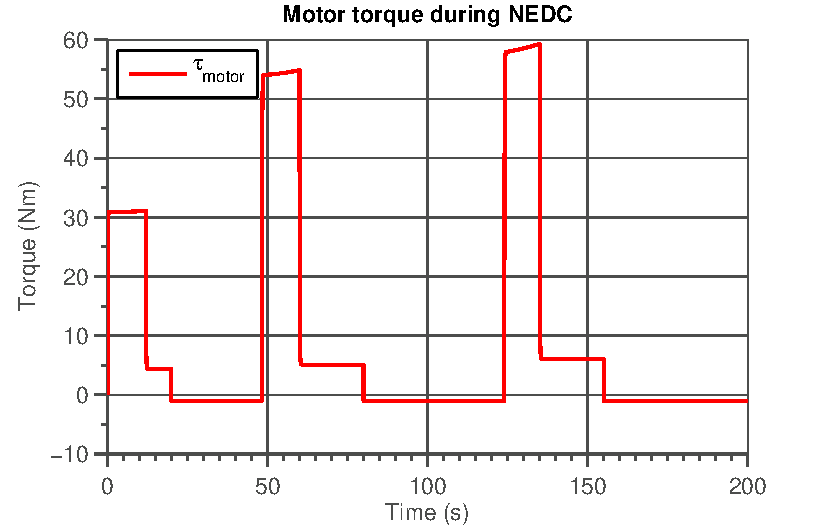
\includegraphics[width=\textwidth]{resource/leaf/torque-motor-rc.pdf}
					\caption{Nissan Leaf Motor Torque}
					\label{fig:ass4-t1-torque-motor}
				\end{subfigure}
				\enspace
				\begin{subfigure}[h]{0.49\textwidth}
					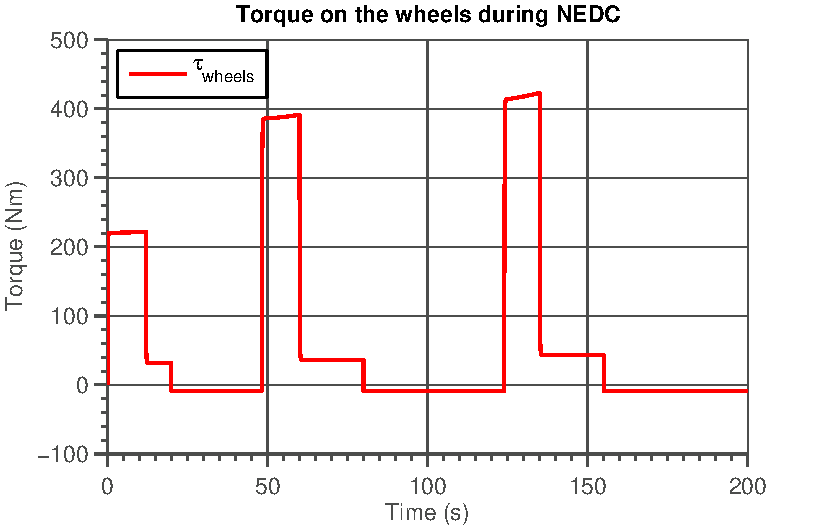
\includegraphics[width=\textwidth]{resource/leaf/torque-wheels-rc.pdf}
					\caption{Nissan Leaf Wheels Torque}
					\label{fig:ass4-t1-torque-wheels}
				\end{subfigure}
			\end{center}
			\caption{Motor and wheels torque on the Nissan Leaf}
			\label{fig:ass4-t1-torque}
		\end{figure}

		\item
		Where torque immediately changes to a relatively constant value, we see motor output power increase very rapidly at first due to the fast increase in torque. (Figure \ref{fig:ass4-t1-motor-bat-power}) After this vehicle velocity becomes the dominant factor to determine motor power, which explains the lower (linear) increase in power. Naturally, battery output power is directly related to motor output power, which explains their respective graphs looking alike so much.

		\begin{figure}[H]
			\begin{center}
				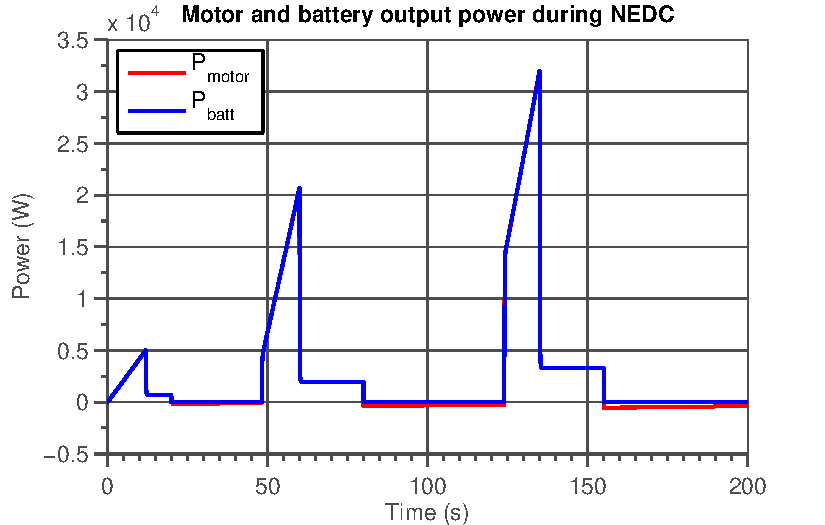
\includegraphics[width=0.6\linewidth]{resource/leaf/motor-bat-power-rc.pdf}
			\end{center}
			\caption{Motor and battery power in generated by the Nissan Leaf}
			\label{fig:ass4-t1-motor-bat-power}
		\end{figure}
	\end{itemize}

\item
	Since aerodynamic drag increases quadratically with vehicle velocity we notice that power also increases approximately quadratically with vehicle velocity. Further, it is worth noticing that, especially at low velocities, driving on a road with \SI{3}{\percent} inclination, requires a lot (about \num{2.75} times) more power than driving on a road without any inclination.

	\begin{figure}[H]
		\begin{center}
			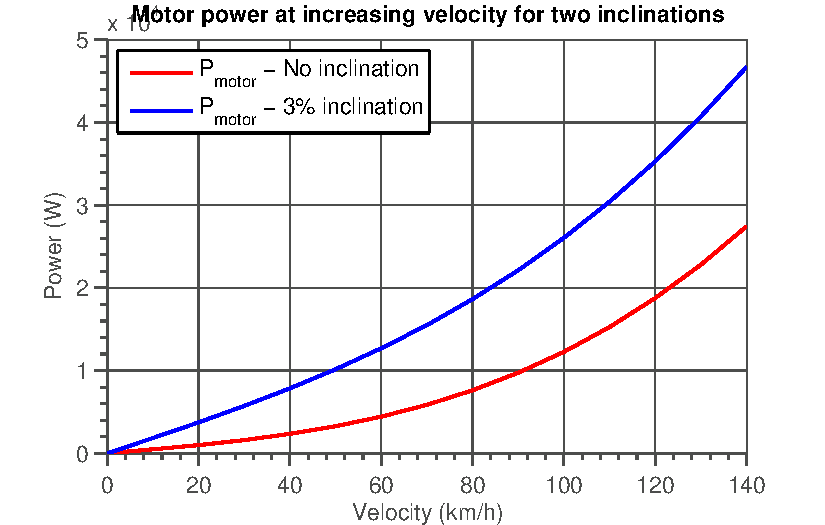
\includegraphics[width=0.6\linewidth]{resource/leaf/power-velocity-rc.pdf}
		\end{center}
		\caption{Motor power and vehicle velocity of a Nissan Leaf}
		\label{fig:ass4-t1-power-velocity}
	\end{figure}

\item
	Because manufacturer claims only hold in optimal conditions, it is safe to say the maximum driving range will only be reached when driving with a very light right foot, without any headwinds, on a perfect road without inclination and in a climate (temperature) that is optimal for battery life.
\end{enumerate}

\section{Task 2}
\begin{enumerate}
\item
	\begin{table}[H]
		\centering
		\caption{Kitt Simulation parameters}
		\label{tab:ass4-sim-param}
		\begin{tabular}{c c}
			\hline\hline
			Parameter & Value \\
			\hline
			Vehicle total mass & \SI{6}{kg} \\
			Wheel diameter & \SI{0.146}{m} \cite{traxxas-datasheet}\\
			Wheel moment of inertia & \SI{0.0032}{kgm^2} \\
			Drivetrain moment of inertia & \SI{7.3}{kgmm^2} \\
			Gear ratio & \num{18.67} \cite{traxxas-datasheet}\\
			Aerodynamic drag coefficient & \SI{0.5}{kg/m} \\
			Vehicle frontal area & \SI{0.024}{m^2} \\
			Rolling resistance coefficient & \num{0.01} \cite{wikipedia-rolling-resistance}\\
			Drivetrain efficiency & \SI{90}{\percent} \\
			\hline
			\end{tabular}
	\end{table}
	These parameters were obtained by various measurements, assumptions, estimations (like the one given in the Student Manual \cite[32]{epo4-manual}) and usage of the equations given in the back of the Student Manual. \cite[119-131]{epo4-manual}

\item
	\begin{table}[H]
		\centering
		\caption{Kitt Simulation parameters}
		\label{tab:ass4-sim-param-cap}
		\begin{tabular}{c c}
			\hline\hline
			Parameter & Value \\
			\hline
			Total capacity & \SI{35}{F} \cite{maxwell-dcell-datasheet} \\
			Max total voltage & \SI{20}{V} \\
			Max total regulator current & \SI{40}{A} \\
			Max total power & \SI{800}{W} \\
			\hline
			\end{tabular}
	\end{table}
\item
	\begin{itemize}
		\item
		Note that for the NEDC-cycle simulations, all velocities have been scaled to a factor of \num{0.3}.
		Comparing Kitt's rolling resistance (Figure \ref{fig:ass4-t1-resistance-friction-kitt}) with the Nissan Leaf's, we spot a difference. Where the Nissan Leaf keeps rolling after the throttle is released, Kitt comes to a full stop a couple of times, due to his smaller momentum. This explains the dips found in the graph. Kitt's aerodynamic drag curve (Figure \ref{fig:ass4-t1-resistance-aero-kitt}) is a bit smoother than the one of the Nissan Leaf, because of the higher drag coefficient.

		\begin{figure}[H]
			\begin{center}
				\begin{subfigure}[h]{0.49\textwidth}
					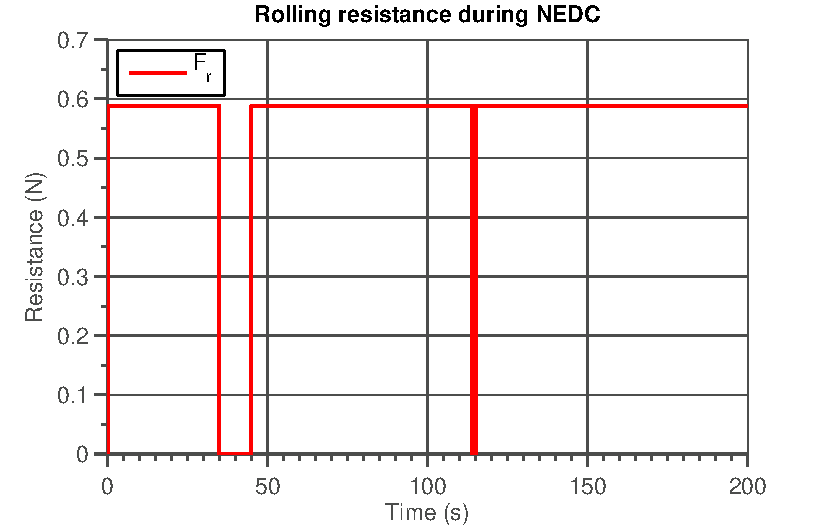
\includegraphics[width=\textwidth]{resource/kitt/resistance-friction-rc.pdf}
					\caption{Kitt's Frictional Resistance}
					\label{fig:ass4-t1-resistance-friction-kitt}
				\end{subfigure}
				\enspace
				\begin{subfigure}[h]{0.49\textwidth}
					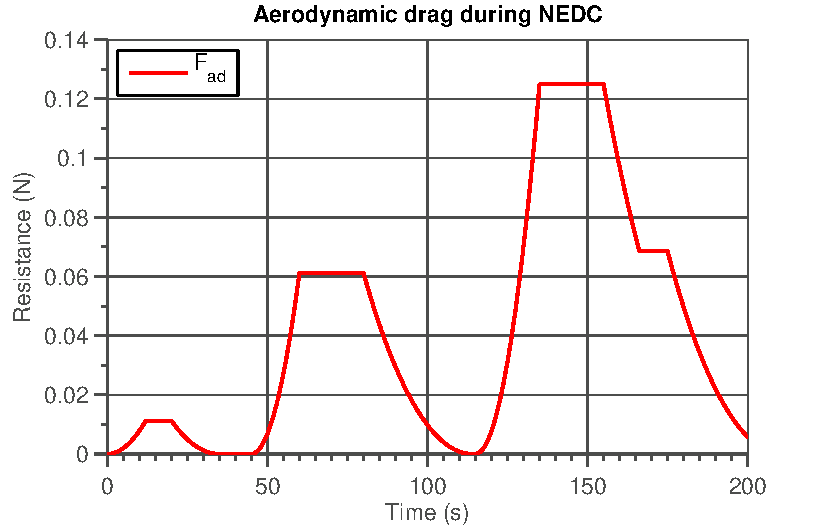
\includegraphics[width=\textwidth]{resource/kitt/resistance-aero-rc.pdf}
					\caption{Kitt's Aerodynamic Drag}
					\label{fig:ass4-t1-resistance-aero-kitt}
				\end{subfigure}
			\end{center}
			\caption{Various resistance forces on Kitt}
			\label{fig:ass4-t1-resistance-kitt}
		\end{figure}

		\item
		Motor and wheel torque (Figure \ref{fig:ass4-t1-torque-kitt}) appear very similair to the Nissan Leaf's, except for the torque during constant velocity, which is larger in proportion to acceleration torque. This is probably due to relatively higher resistive forces on the vehicle.

		\begin{figure}[H]
			\begin{center}
				\begin{subfigure}[h]{0.49\textwidth}
					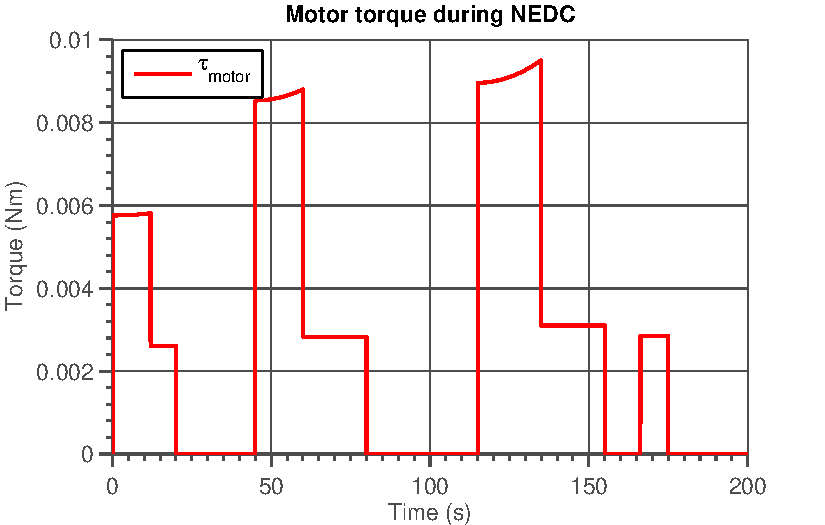
\includegraphics[width=\textwidth]{resource/kitt/torque-motor-rc.pdf}
					\caption{Kitt's Leaf Motor Torque}
					\label{fig:ass4-t1-torque-motor-kitt}
				\end{subfigure}
				\enspace
				\begin{subfigure}[h]{0.49\textwidth}
					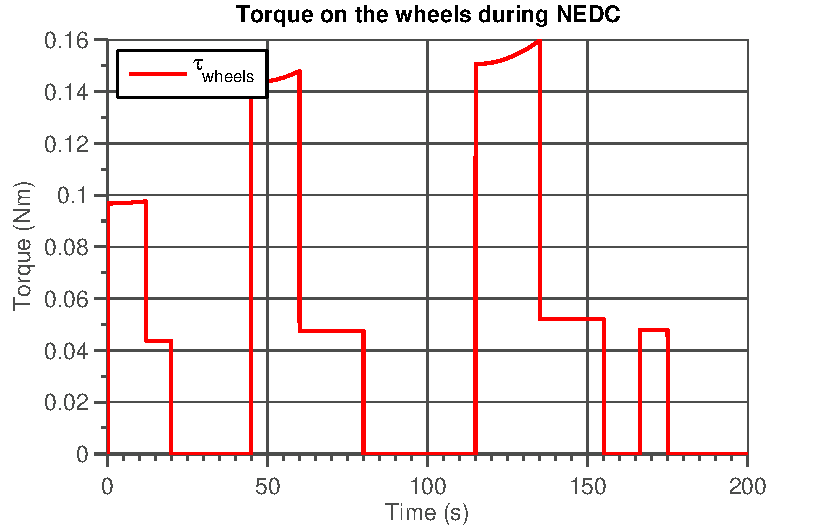
\includegraphics[width=\textwidth]{resource/kitt/torque-wheels-rc.pdf}
					\caption{Kitt's Wheels Torque}
					\label{fig:ass4-t1-torque-wheels-kitt}
				\end{subfigure}
			\end{center}
			\caption{Motor and wheels torque on the Nissan Leaf}
			\label{fig:ass4-t1-torque-kitt}
		\end{figure}

		\item
		In Figure \ref{fig:ass4-t1-motor-bat-power-kitt} we see that vehicle velocity immediately becomes the determining factor for motor and battery power characteristics unlike in the case of the Nissan Leaf. This results from the much lower torque Kitt is able to deliver.

		\begin{figure}[H]
			\begin{center}
				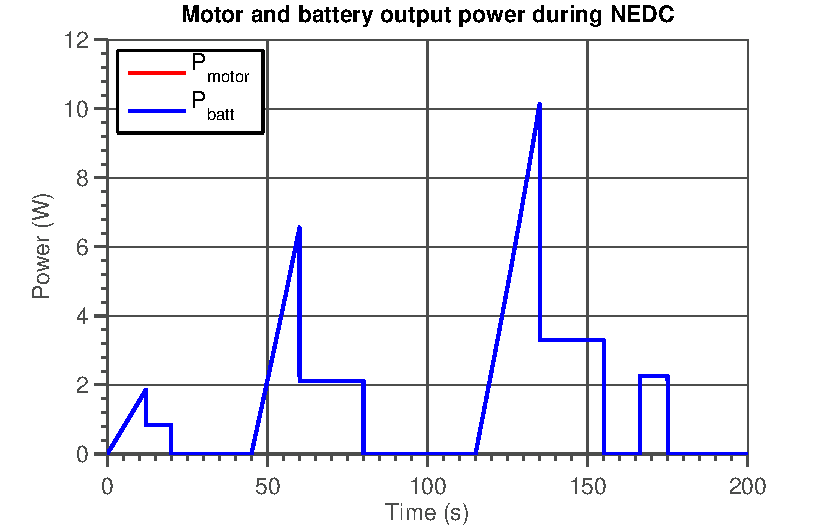
\includegraphics[width=0.6\linewidth]{resource/kitt/motor-bat-power-rc.pdf}
			\end{center}
			\caption{Motor and battery power in generated by Kitt}
			\label{fig:ass4-t1-motor-bat-power-kitt}
		\end{figure}
	\end{itemize}

\item
	In Kitt's velocity-power characteristics (Figure \ref{fig:ass4-t1-power-velocity-kitt}) we observer roughly the same parabolic shape as with the Nissan Leaf. It is, however, a bit flattened out, because of the lower speeds and different torque characteristics.

	\begin{figure}[H]
		\begin{center}
			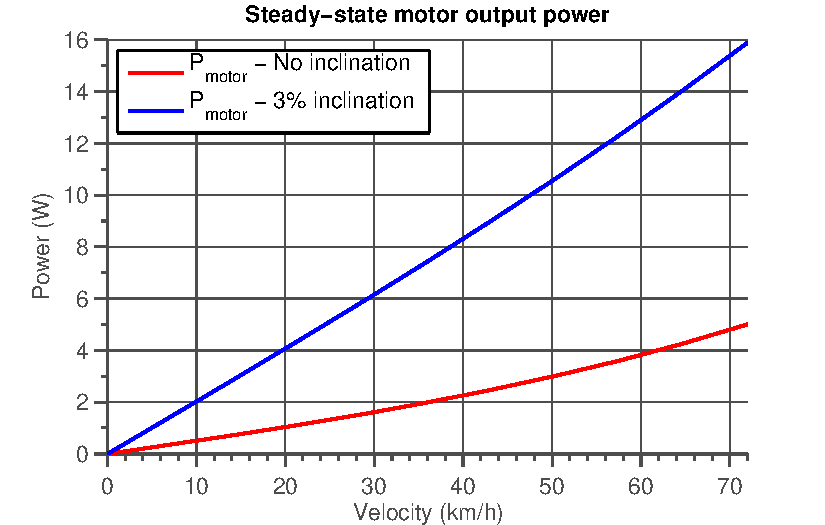
\includegraphics[width=0.6\linewidth]{resource/kitt/power-velocity-rc.pdf}
		\end{center}
		\caption{Motor power and vehicle velocity of Kitt}
		\label{fig:ass4-t1-power-velocity-kitt}
	\end{figure}

\end{enumerate}

\section{Analysis of the forces on a car}
From the motor's perspective, the moment of intertia seen is

\begin{equation}
	J_{eq} = J_m + \frac{1}{N^2} J_L
\end{equation}

in which $N$ represents the gear ratio, $J_m$ the moment of intertia of the motor and $J_L$ the moment of intertia of the load. If an external force, such as air resistance, is applied to the car, then the torque which the motor has to deliver is given by

\begin{equation} \label{eq:ass-4-eq-torque}
	\tau_{m} = \alpha_m (J_m + \frac{1}{N^2} J_L) + \frac{1}{N} \tau_{ex} =
	\frac{a_v N}{r_{wheel}} (J_m + \frac{1}{N^2} J_{wheels}) + r_{wheel} \frac{F_{ex}}{N}.
\end{equation}

Here the acceleration of the moment is denoted by $\alpha_m$, the external torque by $\tau_{ex}$, the acceleration of the vehicle by $a_v$, the radius of the wheels by $r_{wheel}$, the moment of inertia of the wheels by $J_{wheels}$ and the external force by $F_{ex}$. Letting the external force be the aerodynamic drag, gravitational force and rolling resistance yields

\begin{equation}
	\tau_{m} =
	\frac{a_v N}{r_{wheel}} (J_m + \frac{1}{N^2} J_{wheels}) + r_{wheel} \frac{
		m_v g \sin{(\theta)} +
		m_v g \cos{(\theta)} C_r +
		\frac{1}{2} C_w \rho A_f v_{rel}^2
	}{N}.
\end{equation}

Here the rolling resistance coefficient is denoted by $C_r$, the aerodynamic drag coefficient by $C_w$, the mass of the vehicle and passengers by $m_v$, the frontal area by $A_f$, the vehicle's speed relative to the wind $v_{rel}$ and the angle of the inclination of the road by $\theta$. If the power transmission's efficiency is $\eta$ and the vehicle is moving at a speed $v$, then the total power the motor has to deliver is

\begin{equation} \label{eq:ass-3-driving}
	P_{m} = \frac{\omega_m \tau_{m}}{\eta} =
	\frac{N v}{r_{wheel} \eta} \left(
		\frac{a_v N}{r_{wheel}} (J_m + \frac{1}{N^2} J_{wheels}) + r_{wheel} \frac{
			m_v g \sin{(\theta)} +
			m_v g \cos{(\theta)} C_r +
			\frac{1}{2} C_w \rho A_f v_{rel}^2
		}{N}
	\right).
\end{equation}

However, this equation is invalid if the car breaks regeneratively. In this case, the external torque drives the motor. If the efficiency of the power transmission is $\eta_r$, then the power delivered to the motor is given by

\begin{equation} \label{eq:ass-3-regen}
	P_{mr} = \eta_r \omega_m \tau_{m} =
	\frac{N v \eta_r}{r_{wheel}} \left(
		\frac{a_v N}{r_{wheel}} (J_m + \frac{1}{N^2} J_{wheels}) + r_{wheel} \frac{
			m_v g \sin{(\theta)} +
			m_v g \cos{(\theta)} C_r +
			\frac{1}{2} C_w \rho A_f v_{rel}^2
		}{N}
	\right).
\end{equation}

Here the power delivered to the motor is denoted by $P_{mr}$. One should keep in mind that the acceleration of the vehicle should be negative is the vehicle is breaking. Using Equations~\ref{eq:ass-3-driving} and \ref{eq:ass-3-regen}, we were able to solve the questions asked in Exercise 3. We assumed that the rolling resistance coefficient was approximately \num{0.01}, the aerodynamic drag coefficient approximately \num{0.25}, the speed of the wind was \SI{0}{m/s} and there was no inclination of the road. The power needed to for the car to drive at \SI{10}{m/s} and accelerating at \SI{5}{m/s^2} is approximately \SI{4.6}{kW}. The power gained from regenerative breaking with an acceleration of \SI{-2}{m/s} at \SI{30}{m/s} is approximately \SI{6.3}{kW}.

\end{document}